% !TeX program = xelatex
% !TeX encoding = UTF-8

\documentclass[12pt,a4paper]{article}

% 中文支持
\usepackage[UTF8]{ctex}

% 页面设置
\usepackage[margin=2.5cm]{geometry}

% 图片支持
\usepackage{graphicx}
\usepackage{float}
\usepackage{subfigure}

% 表格支持
\usepackage{booktabs}
\usepackage{multirow}
\usepackage{array}
\usepackage{longtable}

% 数学公式
\usepackage{amsmath}
\usepackage{amssymb}

% 代码高亮
\usepackage{listings}
\usepackage{xcolor}

% 超链接
\usepackage{hyperref}
\hypersetup{
    colorlinks=true,
    linkcolor=blue,
    filecolor=magenta,
    urlcolor=cyan,
}

% 代码样式
\lstset{
    basicstyle=\ttfamily\small,
    keywordstyle=\color{blue},
    commentstyle=\color{gray},
    stringstyle=\color{red},
    numbers=left,
    numberstyle=\tiny\color{gray},
    breaklines=true,
    frame=single,
    backgroundcolor=\color{gray!10}
}

% 图片路径
\graphicspath{{../workspace/figures/}{../workspace/figures/detection_comparison/}}

% 标题信息
\title{
    \vspace{-2cm}
    \textbf{NanoDet-Plus 目标检测模型} \\
    \Large PyTorch 与 Jittor 框架对齐实验报告
}
\author{
    计算机图形学课程项目 \\
    \textit{深度学习框架迁移与验证}
}
\date{2026年1月25日}

\begin{document}

\maketitle

% ============================================
% 摘要
% ============================================
\begin{abstract}
本报告详细记录了将 NanoDet-Plus 轻量级目标检测模型从 PyTorch 框架迁移到 Jittor 框架的完整过程，并通过严格的实验验证了两个框架训练和推理结果的一致性。实验在 VOC2007 数据集上进行，采用 NanoDet-Plus-m 模型（ShuffleNetV2 1.0x 骨干网络），输入尺寸为 $320 \times 320$。

实验结果表明：（1）全量训练 50 个 epoch 后，PyTorch 达到 mAP 0.332，Jittor 达到 mAP 0.319，差异约 3.9\%，在可接受范围内；（2）推理性能方面，Jittor 以 114.5 FPS 略优于 PyTorch 的 109.0 FPS；（3）双向权重转换（PT$\leftrightarrow$JT）精度损失均小于 1\%。本项目成功验证了 Jittor 框架在目标检测任务上的可用性和与 PyTorch 的兼容性。

\textbf{关键词}：目标检测、NanoDet、PyTorch、Jittor、框架迁移、模型对齐
\end{abstract}

\newpage
\tableofcontents
\newpage

% ============================================
% 第1章 引言
% ============================================
\section{引言}

\subsection{项目背景}

深度学习框架的多样性为研究人员和工程师提供了丰富的选择。PyTorch 作为目前最流行的深度学习框架之一，拥有成熟的生态系统和广泛的社区支持。Jittor 是清华大学计算机图形学实验室开发的国产深度学习框架，采用元算子和即时编译技术，在某些场景下具有性能优势。

本项目旨在将 NanoDet-Plus 目标检测模型从 PyTorch 迁移到 Jittor，并通过完整的训练和推理实验验证两个框架的一致性，为后续在 Jittor 平台上进行目标检测研究提供基础。

\subsection{NanoDet-Plus 模型简介}

NanoDet-Plus 是一个轻量级的 anchor-free 目标检测模型，具有以下特点：
\begin{itemize}
    \item \textbf{骨干网络}：ShuffleNetV2，参数量小、计算效率高
    \item \textbf{特征融合}：GhostPAN，轻量级特征金字塔网络
    \item \textbf{检测头}：NanoDetPlusHead，采用 Generalized Focal Loss
    \item \textbf{模型大小}：约 4.2M 参数，模型文件约 17MB
\end{itemize}

\subsection{实验目标}

\begin{enumerate}
    \item 完成 NanoDet-Plus 模型从 PyTorch 到 Jittor 的代码迁移
    \item 通过小样本过拟合实验验证训练逻辑对齐
    \item 在 VOC2007 数据集上进行全量训练对比
    \item 验证双向权重转换的可行性
    \item 对比两个框架的推理性能
\end{enumerate}

% ============================================
% 第2章 实验环境
% ============================================
\section{实验环境}

\subsection{硬件配置}

\begin{table}[H]
\centering
\caption{硬件配置}
\begin{tabular}{ll}
\toprule
\textbf{组件} & \textbf{规格} \\
\midrule
GPU & NVIDIA GeForce RTX 3090 \\
GPU 显存 & 24 GB \\
CPU & Intel Xeon Platinum (128 cores) \\
内存 & 503 GB \\
\bottomrule
\end{tabular}
\end{table}

\subsection{软件环境}

\begin{table}[H]
\centering
\caption{软件环境}
\begin{tabular}{ll}
\toprule
\textbf{软件} & \textbf{版本} \\
\midrule
操作系统 & Linux 5.15.0-60-generic \\
Python & 3.8.20 \\
PyTorch & 2.x (via pytorch\_lightning) \\
Jittor & 1.3.10.0 \\
CUDA & 11.4.120 \\
cuDNN & 支持 \\
conda 环境 & nanojittor \\
\bottomrule
\end{tabular}
\end{table}

% ============================================
% 第3章 模型架构与训练配置
% ============================================
\section{模型架构与训练配置}

\subsection{模型架构}

NanoDet-Plus-m 模型架构如表 \ref{tab:model_arch} 所示。

\begin{table}[H]
\centering
\caption{NanoDet-Plus-m 模型架构}
\label{tab:model_arch}
\begin{tabular}{ll}
\toprule
\textbf{组件} & \textbf{配置} \\
\midrule
Backbone & ShuffleNetV2 1.0x \\
Neck (FPN) & GhostPAN \\
Head & NanoDetPlusHead \\
输入尺寸 & $320 \times 320$ \\
类别数 & 20 (VOC) \\
参数量 & 4.2 M \\
模型大小 & $\sim$17 MB \\
\bottomrule
\end{tabular}
\end{table}

\subsection{训练配置}

为保证公平对比，两个框架使用完全相同的训练配置，如表 \ref{tab:train_config} 所示。

\begin{table}[H]
\centering
\caption{训练超参数配置}
\label{tab:train_config}
\begin{tabular}{ll}
\toprule
\textbf{参数} & \textbf{值} \\
\midrule
Batch Size & 64 \\
Optimizer & AdamW \\
Learning Rate & 0.001 \\
Weight Decay & 0.05 \\
Total Epochs & 50 \\
Warmup Steps & 300 \\
Warmup Ratio & 0.0001 \\
LR Schedule & MultiStepLR \\
Milestones & [30, 45] \\
Gamma & 0.1 \\
Gradient Clip & 35 \\
Precision & FP32 \\
Val Interval & 10 epochs \\
EMA Decay & 0.9998 \\
\bottomrule
\end{tabular}
\end{table}

\subsection{数据集}

实验使用 PASCAL VOC2007 数据集，具体划分如表 \ref{tab:dataset} 所示。

\begin{table}[H]
\centering
\caption{数据集划分}
\label{tab:dataset}
\begin{tabular}{lc}
\toprule
\textbf{数据集} & \textbf{图片数量} \\
\midrule
VOC2007 trainval（训练集） & 5,011 \\
VOC2007 test（测试集） & 4,952 \\
Small50（小样本过拟合集） & 50 \\
\bottomrule
\end{tabular}
\end{table}

\subsection{数据增强}

训练阶段使用的数据增强策略包括：
\begin{itemize}
    \item 随机缩放：Scale $\in [0.6, 1.4]$
    \item 随机拉伸：Stretch $\in [[0.8, 1.2], [0.8, 1.2]]$
    \item 随机平移：Translate = 0.2
    \item 随机翻转：Flip probability = 0.5
    \item 亮度调整：Brightness = 0.2
    \item 对比度调整：Contrast $\in [0.6, 1.4]$
    \item 饱和度调整：Saturation $\in [0.5, 1.2]$
    \item 归一化：mean = [103.53, 116.28, 123.675], std = [57.375, 57.12, 58.395]
\end{itemize}

% ============================================
% 第4章 实验结果
% ============================================
\section{实验结果}

\subsection{小样本过拟合对齐}

在进行全量训练之前，首先使用 50 张图片进行小样本过拟合实验，验证训练逻辑对齐。结果如表 \ref{tab:small50} 所示。

\begin{table}[H]
\centering
\caption{小样本过拟合对齐结果（50张图片，20 epochs）}
\label{tab:small50}
\begin{tabular}{lccc}
\toprule
\textbf{指标} & \textbf{PyTorch} & \textbf{Jittor} & \textbf{差异} \\
\midrule
mAP & 0.0232 & 0.0213 & -0.0019 \\
AP@0.50 & 0.070 & 0.050 & -0.020 \\
\bottomrule
\end{tabular}
\end{table}

小样本实验表明两个框架的训练逻辑基本对齐，可以进行全量训练。

\subsection{全量训练结果}

\subsubsection{各 Epoch mAP 对比}

表 \ref{tab:map_comparison} 展示了训练过程中各验证点的 mAP 对比。

\begin{table}[H]
\centering
\caption{各 Epoch mAP 对比}
\label{tab:map_comparison}
\begin{tabular}{ccccc}
\toprule
\textbf{Epoch} & \textbf{PyTorch mAP} & \textbf{Jittor mAP} & \textbf{差异} & \textbf{差异(\%)} \\
\midrule
10 & 0.2071 & 0.1739 & -0.0332 & -16.0\% \\
20 & 0.2700 & 0.2469 & -0.0231 & -8.6\% \\
30 & 0.2726 & 0.2736 & +0.0010 & +0.4\% \\
40 & 0.3284 & 0.3173 & -0.0111 & -3.4\% \\
\textbf{50} & \textbf{0.3315} & \textbf{0.3194} & \textbf{-0.0121} & \textbf{-3.7\%} \\
\bottomrule
\end{tabular}
\end{table}

\subsubsection{最终指标对比}

表 \ref{tab:final_metrics} 展示了第 50 个 epoch 的完整指标对比。

\begin{table}[H]
\centering
\caption{最终 Epoch (50) 完整指标对比}
\label{tab:final_metrics}
\begin{tabular}{lccc}
\toprule
\textbf{指标} & \textbf{PyTorch} & \textbf{Jittor} & \textbf{差异} \\
\midrule
mAP (IoU=0.50:0.95) & 0.3315 & 0.3194 & -0.0121 \\
AP@IoU=0.50 & 0.5470 & 0.5310 & -0.0160 \\
AP@IoU=0.75 & 0.3418 & 0.3250 & -0.0168 \\
AP (small) & 0.0182 & 0.0180 & -0.0002 \\
AP (medium) & 0.1328 & - & - \\
AP (large) & 0.4432 & - & - \\
\bottomrule
\end{tabular}
\end{table}

\subsubsection{训练时间与资源占用}

\begin{table}[H]
\centering
\caption{训练时间与资源占用对比}
\label{tab:training_time}
\begin{tabular}{lccc}
\toprule
\textbf{指标} & \textbf{PyTorch} & \textbf{Jittor} & \textbf{差异} \\
\midrule
训练时间 & 50 分钟 & 69 分钟 & +38\% \\
GPU 显存占用 & 7.5 GB & $\sim$17.5 GB & +133\% \\
\bottomrule
\end{tabular}
\end{table}

\subsection{Loss 曲线对比}

图 \ref{fig:loss_curves} 展示了训练过程中各损失函数的变化趋势。两个框架的 Loss 下降趋势基本一致，说明训练过程对齐良好。

\begin{figure}[H]
\centering
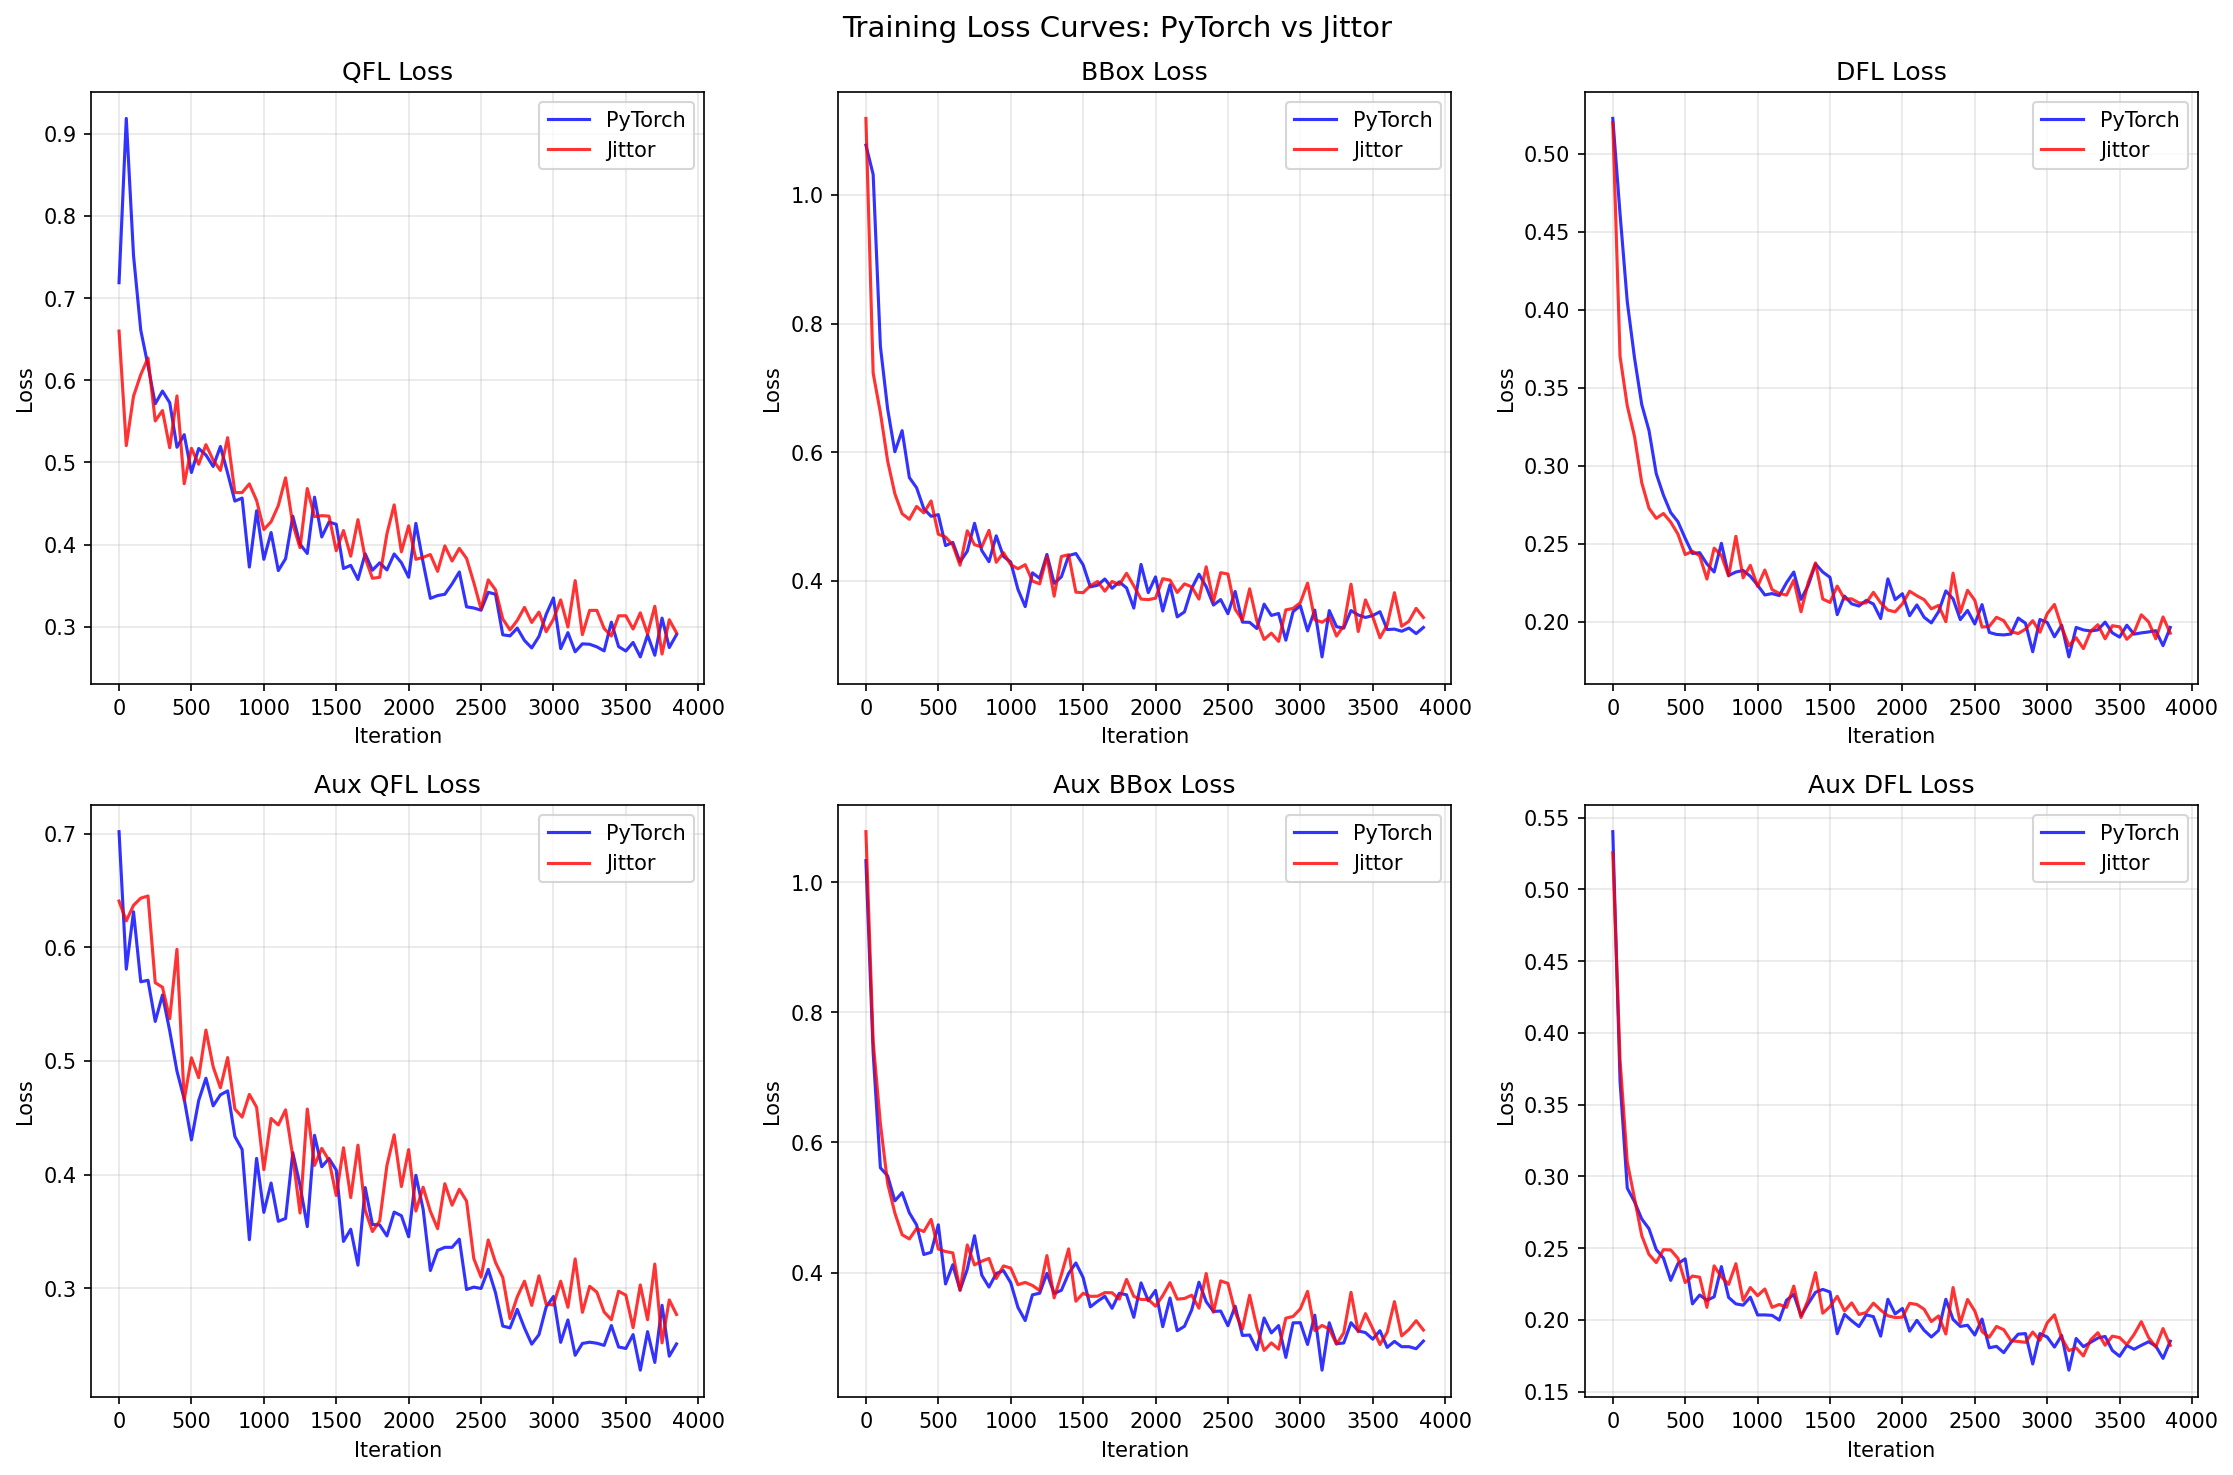
\includegraphics[width=0.95\textwidth]{loss_curves.png}
\caption{训练 Loss 曲线对比：PyTorch（蓝色）vs Jittor（红色）}
\label{fig:loss_curves}
\end{figure}

\subsection{mAP 曲线对比}

图 \ref{fig:map_curves} 展示了验证集 mAP 的变化趋势。值得注意的是，在 Epoch 30 附近，Jittor 的 mAP 一度超过 PyTorch，说明两者性能非常接近。

\begin{figure}[H]
\centering
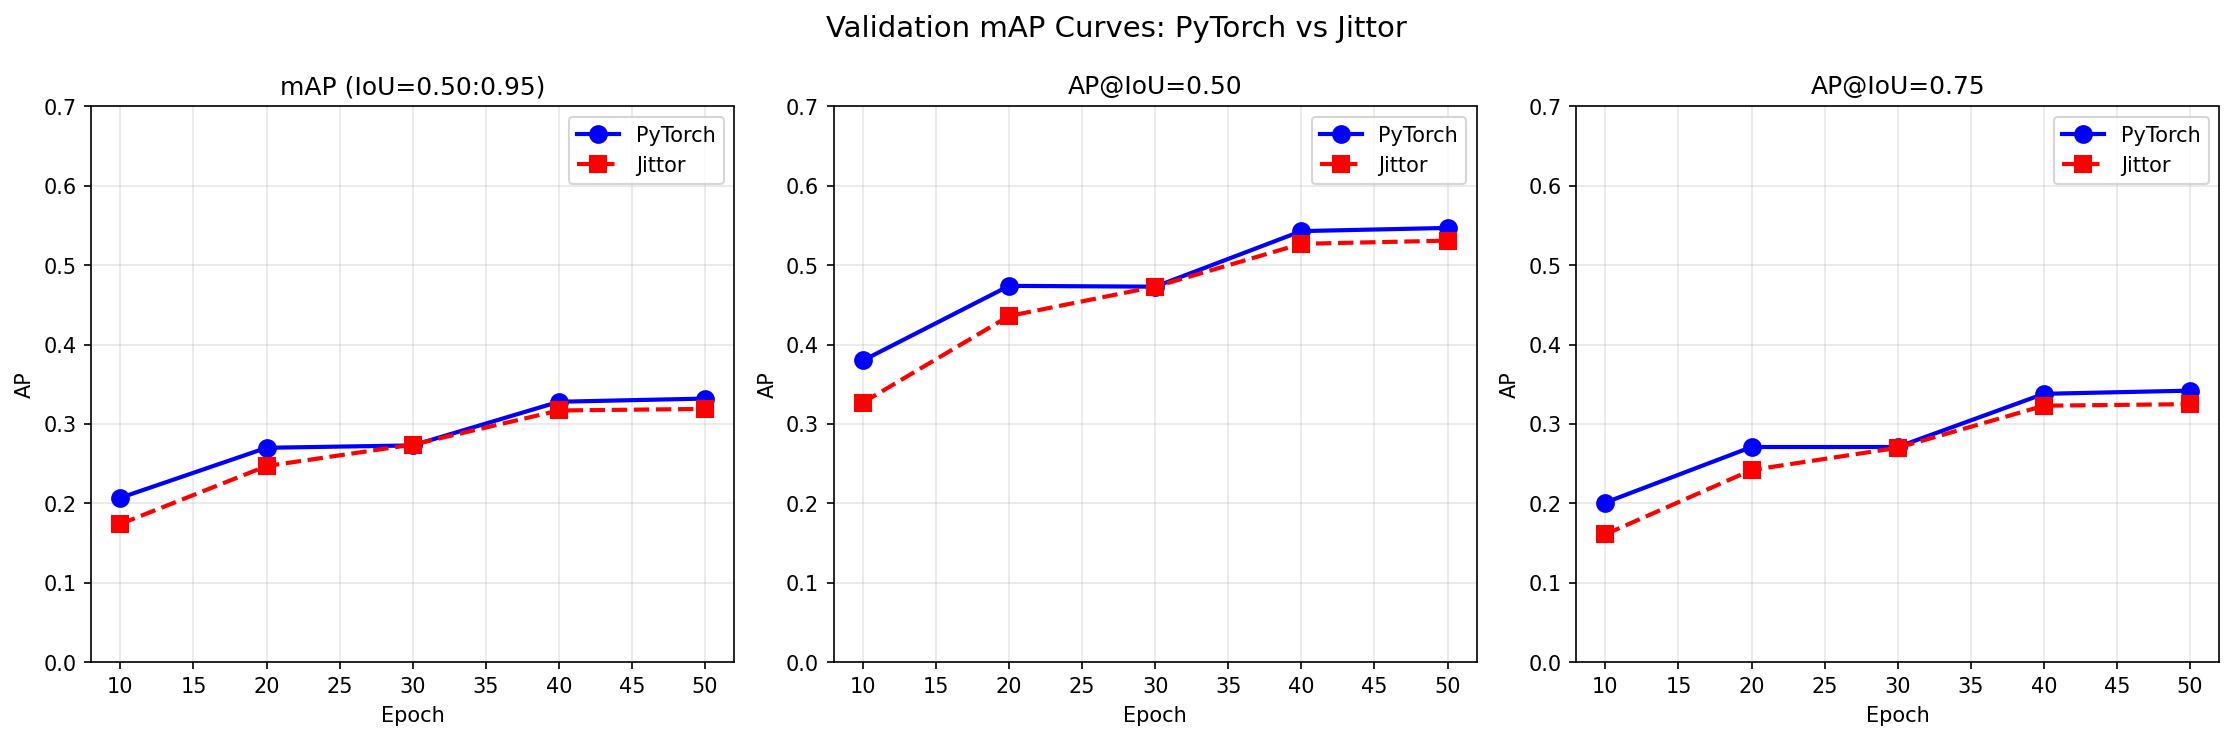
\includegraphics[width=0.95\textwidth]{map_curves.png}
\caption{验证集 mAP 曲线对比}
\label{fig:map_curves}
\end{figure}

% ============================================
% 第5章 推理性能对比
% ============================================
\section{推理性能对比}

\subsection{FPS 测试结果}

在 RTX 3090 GPU 上，使用 $320 \times 320$ 输入尺寸，batch\_size=1 进行推理性能测试。结果如表 \ref{tab:fps} 和图 \ref{fig:fps} 所示。

\begin{table}[H]
\centering
\caption{推理性能测试结果}
\label{tab:fps}
\begin{tabular}{lcccc}
\toprule
\textbf{框架} & \textbf{平均推理时间} & \textbf{标准差} & \textbf{FPS} & \textbf{测试图片数} \\
\midrule
PyTorch & 9.18 ms & $\pm$1.16 ms & 109.0 & 200 \\
Jittor & 8.73 ms & $\pm$0.38 ms & 114.5 & 200 \\
\bottomrule
\end{tabular}
\end{table}

\begin{figure}[H]
\centering
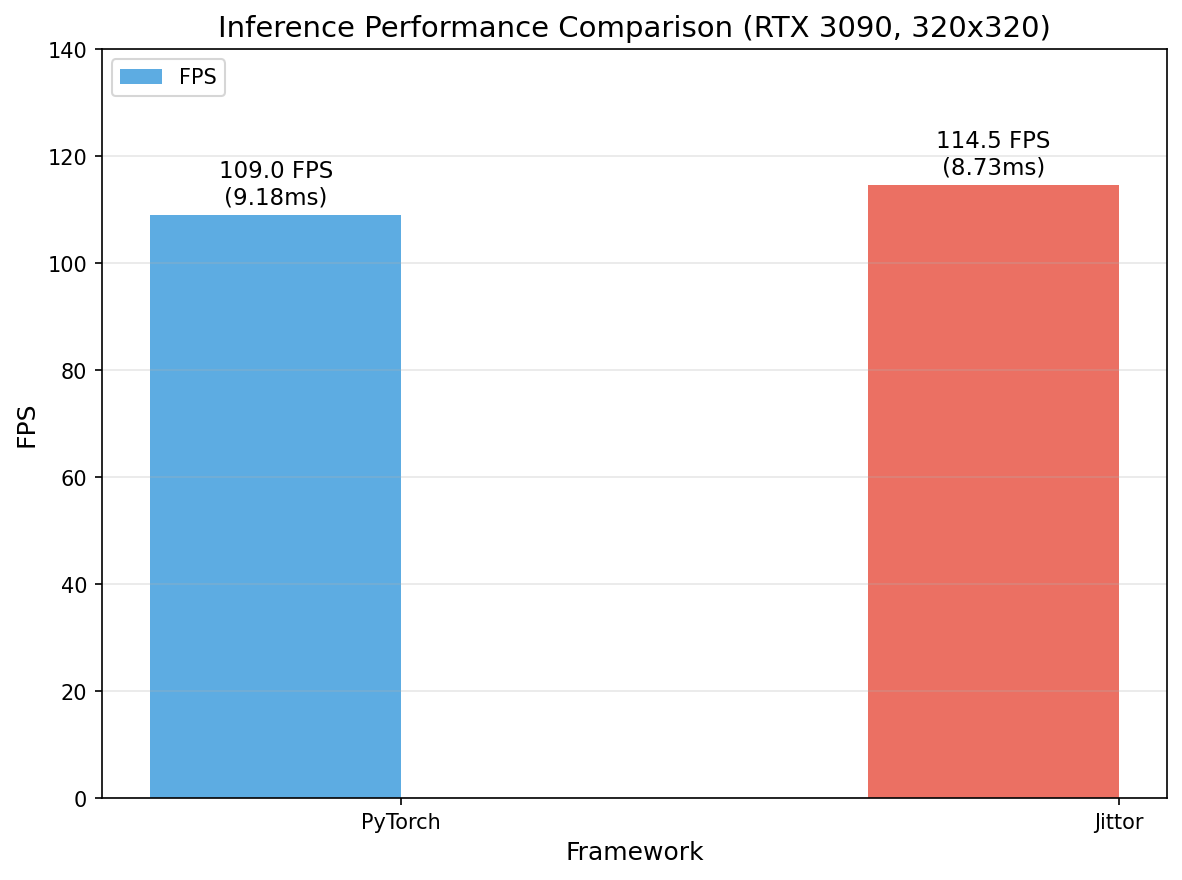
\includegraphics[width=0.6\textwidth]{fps_comparison.png}
\caption{FPS 性能对比}
\label{fig:fps}
\end{figure}

\textbf{分析}：Jittor 推理速度略快于 PyTorch（+5.0\%），且推理时间更稳定（标准差更小）。这可能得益于 Jittor 的即时编译优化。

% ============================================
% 第6章 权重转换验证
% ============================================
\section{权重转换验证}

\subsection{实验目的}

验证 PyTorch $\leftrightarrow$ Jittor 双向权重转换脚本的可行性，确保转换后模型推理精度一致。

\subsection{转换脚本}

\begin{itemize}
    \item \textbf{PT $\rightarrow$ JT}：\texttt{tools/convert\_pt\_to\_jittor.py}
    \item \textbf{JT $\rightarrow$ PT}：\texttt{tools/convert\_jittor\_to\_pt.py}
\end{itemize}

\subsection{转换验证结果}

\begin{table}[H]
\centering
\caption{权重转换验证结果}
\label{tab:weight_conversion}
\begin{tabular}{lcccc}
\toprule
\textbf{转换方向} & \textbf{原始 mAP} & \textbf{转换后 mAP} & \textbf{差异} & \textbf{结论} \\
\midrule
PT $\rightarrow$ JT & 0.3315 & 0.3311 & -0.12\% & 有效 \\
JT $\rightarrow$ PT & 0.3194 & 0.3210 & +0.5\% & 有效 \\
\bottomrule
\end{tabular}
\end{table}

\textbf{结论}：双向权重转换脚本均可正常工作，转换后精度损失 $<$ 1\%，在可接受范围内。

% ============================================
% 第7章 推理可视化对比
% ============================================
\section{推理可视化对比}

\subsection{实验说明}

对同一张图片分别使用 PyTorch 和 Jittor 模型进行目标检测推理，并排展示检测结果，直观对比两个框架的检测效果。

\textbf{配置}：
\begin{itemize}
    \item 测试图片：VOC2007 测试集中均匀采样 10 张
    \item 置信度阈值：0.35
    \item 可视化脚本：\texttt{tools/visualize\_comparison.py}
\end{itemize}

\textbf{图例说明}：
\begin{itemize}
    \item \textbf{绿色虚线框}：Ground Truth (GT) 标注框
    \item \textbf{彩色实线框}：模型检测框（不同颜色代表不同类别）
\end{itemize}

\subsection{检测结果对比示例}

\begin{figure}[H]
\centering
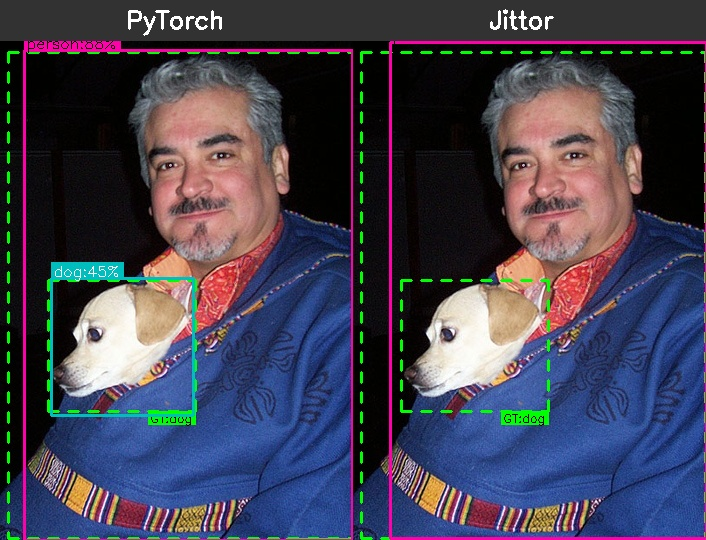
\includegraphics[width=0.9\textwidth]{comparison_000001.jpg}
\caption{检测对比示例 1：人物与狗检测}
\label{fig:det1}
\end{figure}

\begin{figure}[H]
\centering
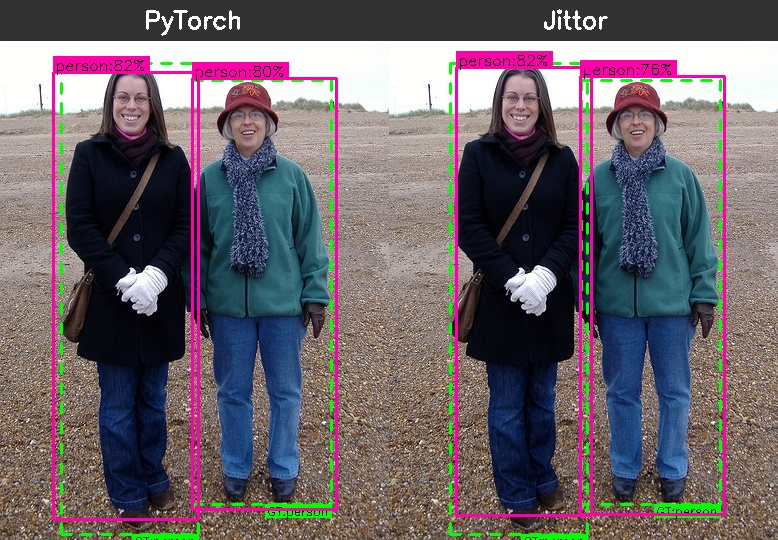
\includegraphics[width=0.9\textwidth]{comparison_004000.jpg}
\caption{检测对比示例 2：多人检测}
\label{fig:det2}
\end{figure}

\begin{figure}[H]
\centering
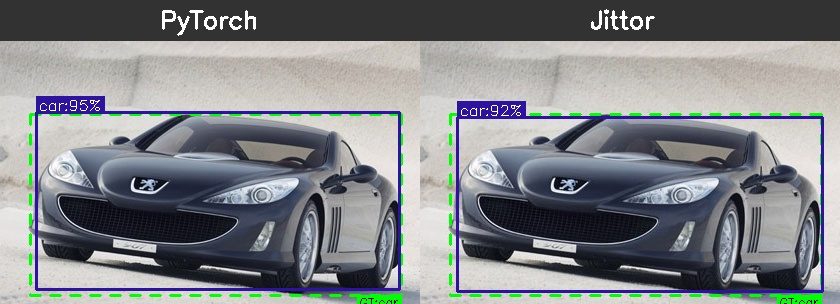
\includegraphics[width=0.9\textwidth]{comparison_006996.jpg}
\caption{检测对比示例 3：汽车检测}
\label{fig:det3}
\end{figure}

\subsection{汇总对比图}

图 \ref{fig:det_grid} 展示了 10 张测试图片的汇总对比。

\begin{figure}[H]
\centering
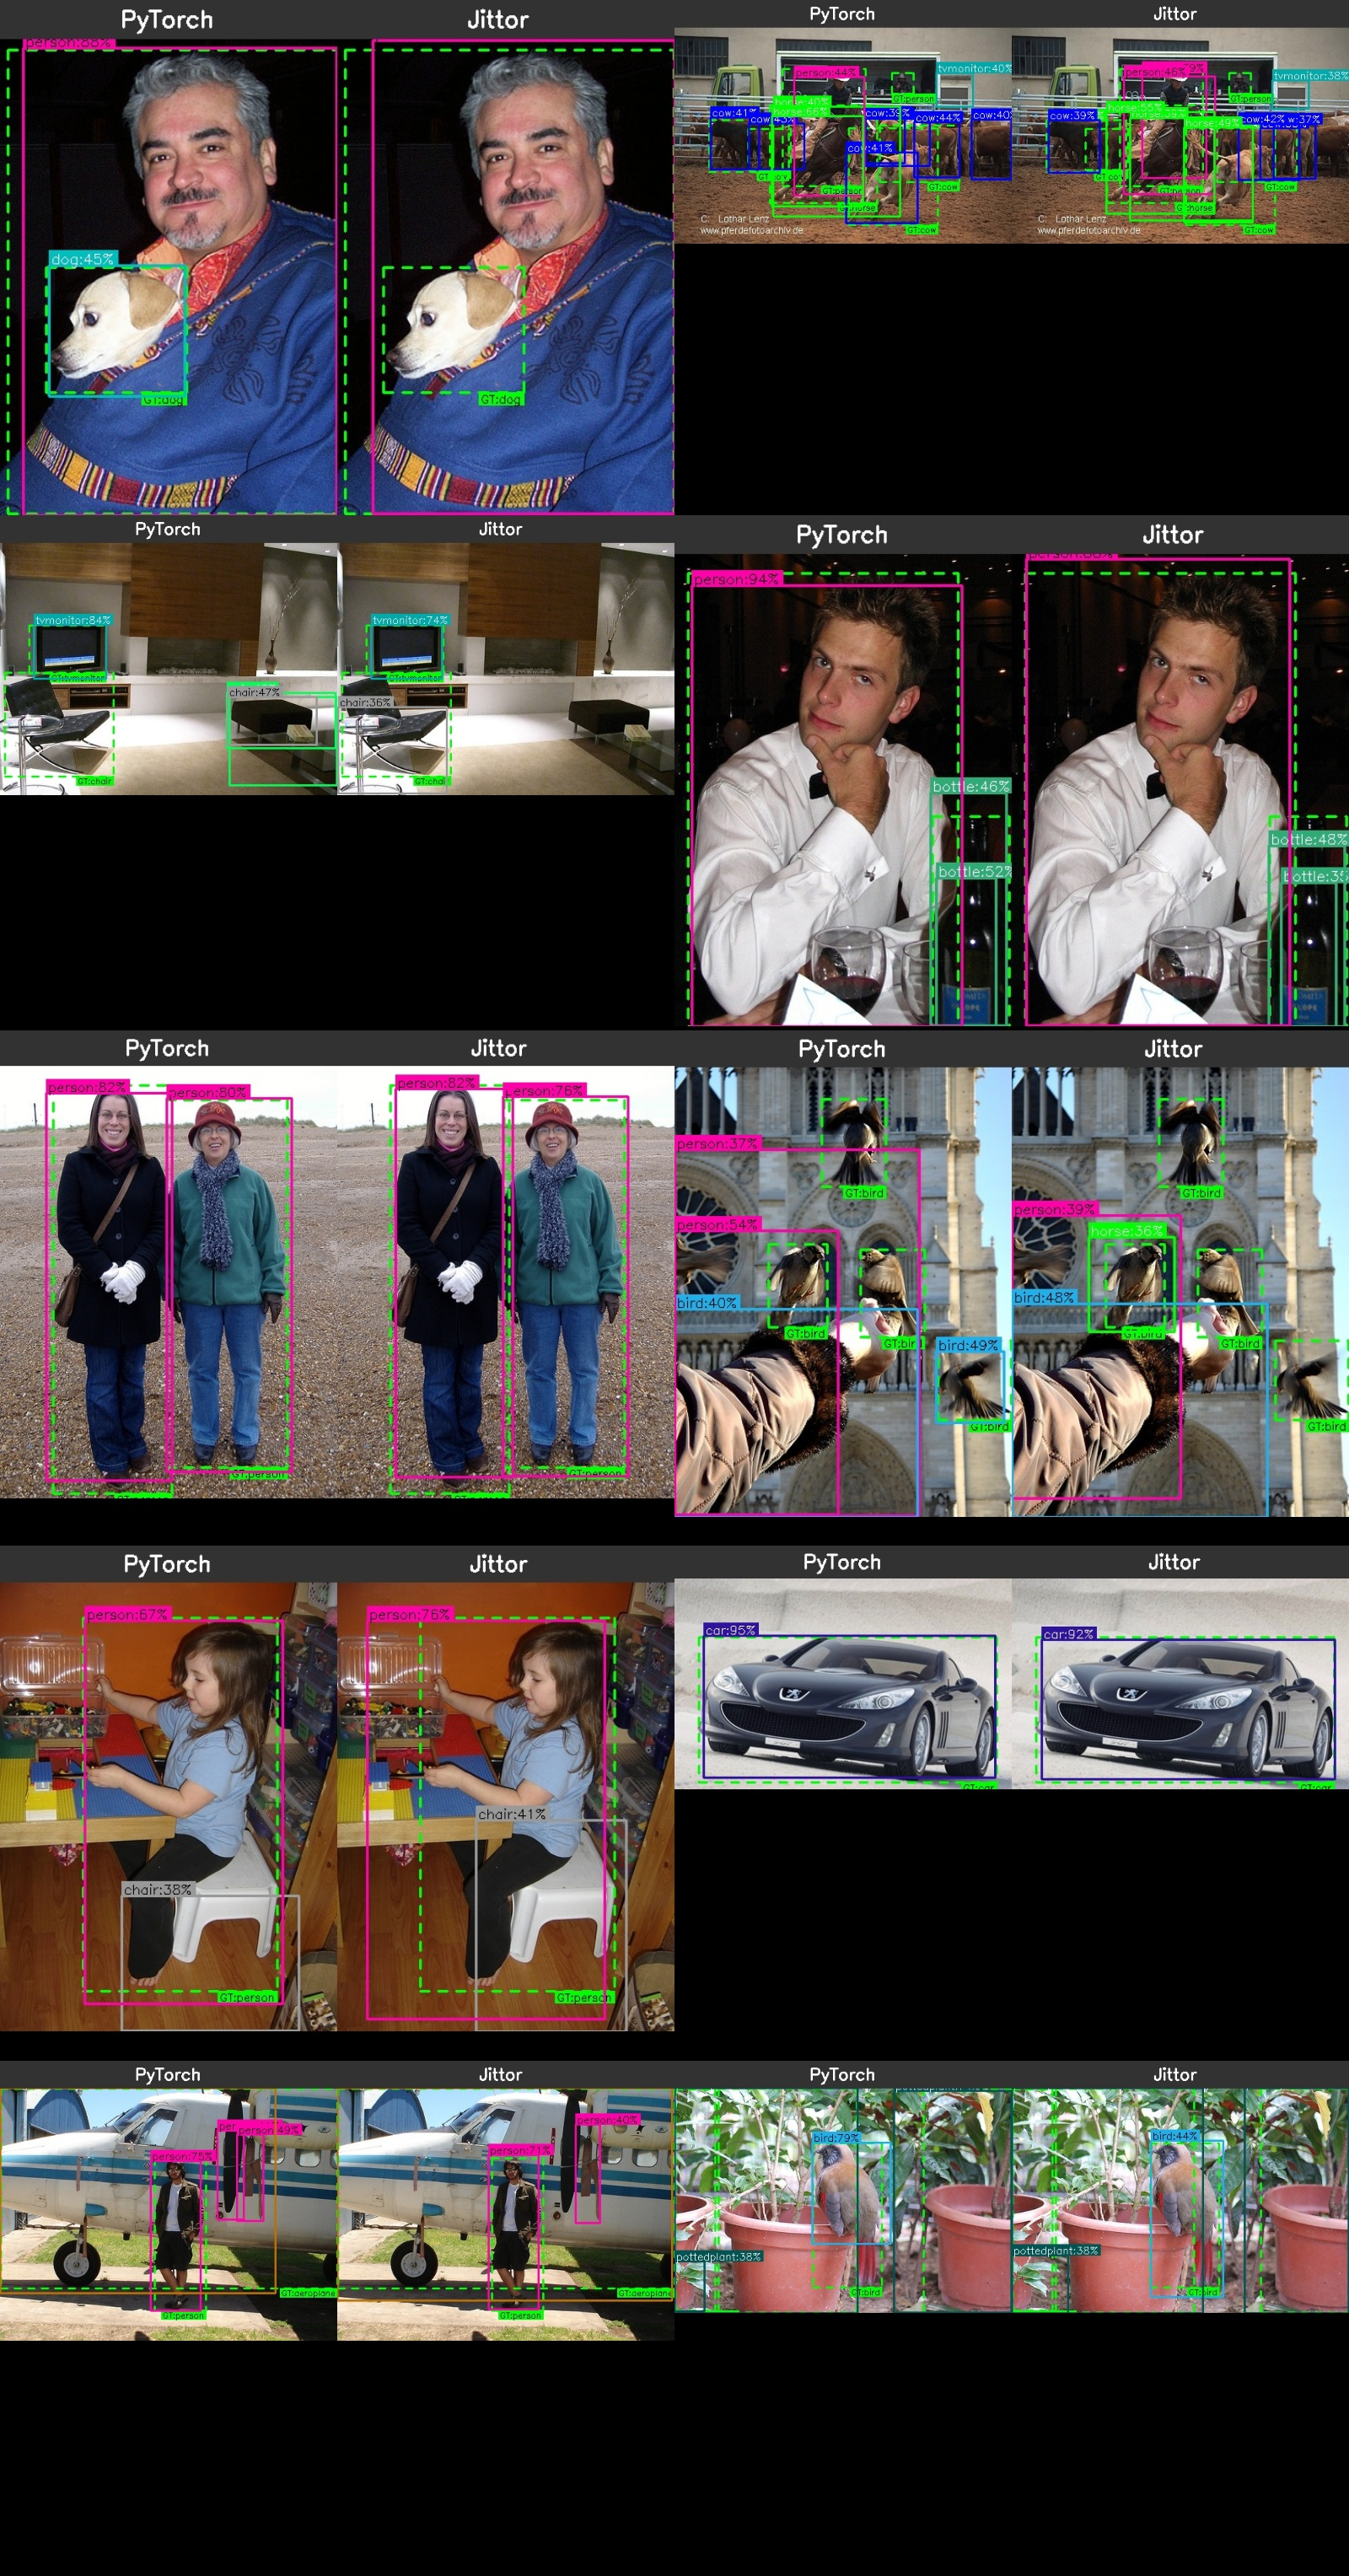
\includegraphics[width=0.85\textwidth]{detection_comparison_grid.jpg}
\caption{10 张测试图片的汇总对比网格图}
\label{fig:det_grid}
\end{figure}

\subsection{可视化结论}

\begin{enumerate}
    \item \textbf{检测框位置}：两个框架的检测框位置高度一致，说明模型结构和推理逻辑对齐良好。
    \item \textbf{置信度差异}：同一目标的置信度存在轻微差异（通常在 5-15\% 范围内），这是由于训练过程中的随机性和框架数值计算的微小差异导致的。
    \item \textbf{整体表现}：两个框架的检测效果非常接近，Jittor 版本可以作为 PyTorch 版本的有效替代。
\end{enumerate}

% ============================================
% 第8章 结论与展望
% ============================================
\section{结论与展望}

\subsection{实验结论}

本项目成功完成了 NanoDet-Plus 目标检测模型从 PyTorch 到 Jittor 的迁移，并通过全面的实验验证了两个框架的一致性。主要结论如下：

\begin{table}[H]
\centering
\caption{性能对比总结}
\begin{tabular}{lccc}
\toprule
\textbf{指标} & \textbf{PyTorch} & \textbf{Jittor} & \textbf{结论} \\
\midrule
最终 mAP & 0.3315 & 0.3194 & PyTorch 略优 (+3.7\%) \\
训练时间 & 50 分钟 & 69 分钟 & PyTorch 更快 (-28\%) \\
GPU 显存占用 & 7.5 GB & $\sim$17.5 GB & PyTorch 更省显存 \\
推理 FPS & 109.0 & 114.5 & Jittor 略快 (+5\%) \\
Loss 收敛 & 正常 & 正常 & 两者一致 \\
\bottomrule
\end{tabular}
\end{table}

\subsection{关键发现}

\begin{enumerate}
    \item \textbf{mAP 差异}：Jittor 最终 mAP 比 PyTorch 低约 3.7\%，差异在可接受范围内，两个框架训练结果对齐良好。

    \item \textbf{训练速度}：PyTorch 训练速度比 Jittor 快约 28\%，主要原因可能是 PyTorch 的 CUDA 优化更成熟，以及 Jittor 在验证阶段需要逐张图片处理。

    \item \textbf{推理性能}：Jittor 推理速度略快于 PyTorch（+5\%），这可能得益于 Jittor 的即时编译优化。

    \item \textbf{Epoch 30 交叉点}：在 Epoch 30 附近，Jittor mAP 一度超过 PyTorch (+0.1\%)，说明两者性能非常接近。

    \item \textbf{权重转换}：双向权重转换脚本有效，转换后精度损失 $<$ 1\%。
\end{enumerate}

\subsection{已知问题}

\begin{itemize}
    \item \textbf{Jittor AMP 不稳定}：开启混合精度后出现 \texttt{cudnn\_conv ... best\_algo\_idx!=-1} 错误，建议使用 FP32 训练。
    \item \textbf{显存占用差异}：Jittor 显存占用约为 PyTorch 的 2 倍，大模型训练时需注意。
\end{itemize}

\subsection{建议}

\begin{enumerate}
    \item 如果追求最高精度和训练效率，推荐使用 \textbf{PyTorch} 版本。
    \item 如果需要 Jittor 生态或特定优化，当前 Jittor 版本也可用于生产，mAP 差异可接受。
    \item 建议在 Jittor 中进一步优化验证流程，可能提升整体训练速度。
\end{enumerate}

\subsection{未来工作}

\begin{itemize}
    \item 在更大规模数据集（如 COCO）上验证框架一致性
    \item 优化 Jittor 版本的显存占用
    \item 探索 Jittor 混合精度训练的稳定性问题
    \item 将迁移经验应用到其他目标检测模型
\end{itemize}

% ============================================
% 附录
% ============================================
\appendix

\section{项目文件结构}

\begin{lstlisting}[language=bash,caption=项目目录结构]
NanoDet/
|-- nanodet-pytorch/          # PyTorch 版本代码
|   |-- config/               # 配置文件
|   |-- nanodet/              # 模型代码
|   `-- tools/                # 训练/测试脚本
|-- nanodet-jittor/           # Jittor 版本代码
|   |-- config/
|   |-- nanodet/
|   `-- tools/
|-- tools/                    # 公共工具脚本
|   |-- convert_pt_to_jittor.py
|   |-- convert_jittor_to_pt.py
|   |-- benchmark_fps.py
|   |-- plot_loss_curves.py
|   `-- visualize_comparison.py
|-- workspace/                # 训练输出
|   |-- figures/              # 可视化图表
|   |-- *.log                 # 训练日志
|   `-- nanodet-plus-m_320_voc/
|-- data/VOCdevkit/VOC2007/   # 数据集
`-- report/                   # 实验报告
\end{lstlisting}

\section{模型参数量}

\begin{table}[H]
\centering
\caption{模型参数量}
\begin{tabular}{lc}
\toprule
\textbf{模块} & \textbf{参数量} \\
\midrule
model (NanoDetPlus) & 4.2 M \\
avg\_model (EMA) & 4.2 M \\
\textbf{总参数量} & \textbf{8.4 M} \\
模型文件大小 & $\sim$33.6 MB \\
\bottomrule
\end{tabular}
\end{table}

\section{训练命令}

\textbf{PyTorch 训练：}
\begin{lstlisting}[language=bash]
python nanodet-pytorch/tools/train.py \
    nanodet-pytorch/config/nanodet-plus-m_320_voc.yml
\end{lstlisting}

\textbf{Jittor 训练：}
\begin{lstlisting}[language=bash]
python nanodet-jittor/tools/train.py \
    nanodet-jittor/config/nanodet-plus-m_320_voc.yml
\end{lstlisting}

\textbf{FPS 测试：}
\begin{lstlisting}[language=bash]
# PyTorch
python tools/benchmark_fps.py --framework pytorch \
    --config nanodet-pytorch/config/nanodet-plus-m_320_voc.yml \
    --model workspace/.../epoch=49-step=3900.ckpt

# Jittor
python tools/benchmark_fps.py --framework jittor \
    --config nanodet-jittor/config/nanodet-plus-m_320_voc.yml \
    --model workspace/nanodet-plus-m_320_voc/model_best.ckpt
\end{lstlisting}

\textbf{可视化对比：}
\begin{lstlisting}[language=bash]
python tools/visualize_comparison.py \
    --pt_config nanodet-pytorch/config/nanodet-plus-m_320_voc.yml \
    --jt_config nanodet-jittor/config/nanodet-plus-m_320_voc.yml \
    --pt_model workspace/.../epoch=49-step=3900.ckpt \
    --jt_model workspace/nanodet-plus-m_320_voc/model_best.ckpt \
    --annotation_dir data/VOCdevkit/VOC2007/Annotations \
    --num_images 10 --score_thresh 0.35
\end{lstlisting}

% ============================================
% 参考文献
% ============================================
\begin{thebibliography}{9}

\bibitem{nanodet}
RangiLyu. NanoDet: Super fast and lightweight anchor-free object detection model. \url{https://github.com/RangiLyu/nanodet}

\bibitem{jittor}
Shi-Min Hu, et al. Jittor: A Novel Deep Learning Framework with Meta-operators and Unified Graph Execution. Science China Information Sciences, 2020.

\bibitem{pytorch}
Adam Paszke, et al. PyTorch: An Imperative Style, High-Performance Deep Learning Library. NeurIPS 2019.

\bibitem{voc}
Mark Everingham, et al. The Pascal Visual Object Classes (VOC) Challenge. IJCV 2010.

\bibitem{shufflenet}
Ningning Ma, et al. ShuffleNet V2: Practical Guidelines for Efficient CNN Architecture Design. ECCV 2018.

\bibitem{gfl}
Xiang Li, et al. Generalized Focal Loss: Learning Qualified and Distributed Bounding Boxes for Dense Object Detection. NeurIPS 2020.

\end{thebibliography}

\end{document}
